\documentclass[11pt]{article}
\usepackage{latexsym}
\usepackage{natbib}
\usepackage{graphicx}
\usepackage{caption}
\usepackage{subcaption}
\usepackage{listings}
\usepackage{algorithm}
\usepackage{algpseudocode}

\title{Homework 5: Reinforcement Learning}
\author{Shun Zhang}
\date{}

\begin{document}
\maketitle

\section{Q-Learning}

Q-Learning is an off-policy temporal difference learning algorithm. It
keeps a Q-table which evaluates each state, action pair. The idea is
to update Q-values with the observed sample, with the learning rate of
$\alpha$, shown in the equation below.

$$Q(s, a) = (1 - \alpha) Q(s, a) + \alpha (r + \gamma Q(s', a'))$$

In this assignment, I need to extract features in the domains. For
example, I represent the states by the distance to the nearest
obstacle in the obstacle domain (will be described in the experiment
section). Let $f_i$ be the i-th feature, and $w_i$ be the weight of
the i-th feature, the Q function can be represented as

$$Q(s, a) = \sum w_i f_i(s, a)$$

To update $Q(s, a)$, $w_i$ needs to be updated. As $\frac{\partial
Q(s, a)}{\partial w_i} = f_i(s, a)$, the update machanism can be
changed to be as follows.

$$correction = r + \gamma Q(s', a') - Q(s, a)$$
$$w_i = w_i + \alpha [correction] f_i(s, a)$$

\section{Modular RL}

\subsection{Linear Combination}

One easy way to mix sub-MPDs is represent the Q-value of the hybird
MDP as linear combination as sub-MDPs. That is,
$$Q(s, a) = \sum{\beta_i Q_i(s, a)}$$
where $\beta_i$ is the weight on the i-th sub-MDP. $Q_i$ is the
Q-value of the i-th sub-MDP.

\subsection{Gibbs Softmax}

The motivation is to normalize the Q-values over the actions given a
state.

$$Q'_i(s, a) = \frac{e^{Q_i(s, a)}}{\sum\limits_{a \in A(s)}e^{Q_i(s, a)}}$$
$$Q(s, a) = \sum{\beta_i Q'_i(s, a)}$$
where $A(s)$ is the set of available actions in the state $s$.
$Q'_i$ is the normalized Q-value.

\section{Experiments}

\begin{figure}[h!]
\centering
\begin{subfigure}{0.9\textwidth}
	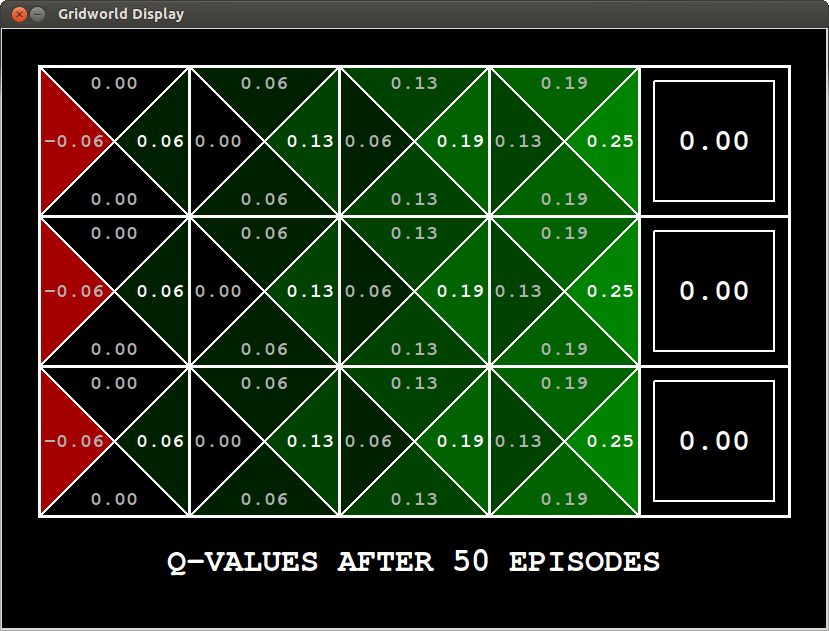
\includegraphics[width=\textwidth]{figure/sidewalk}
\end{subfigure}
\begin{subfigure}{0.9\textwidth}
	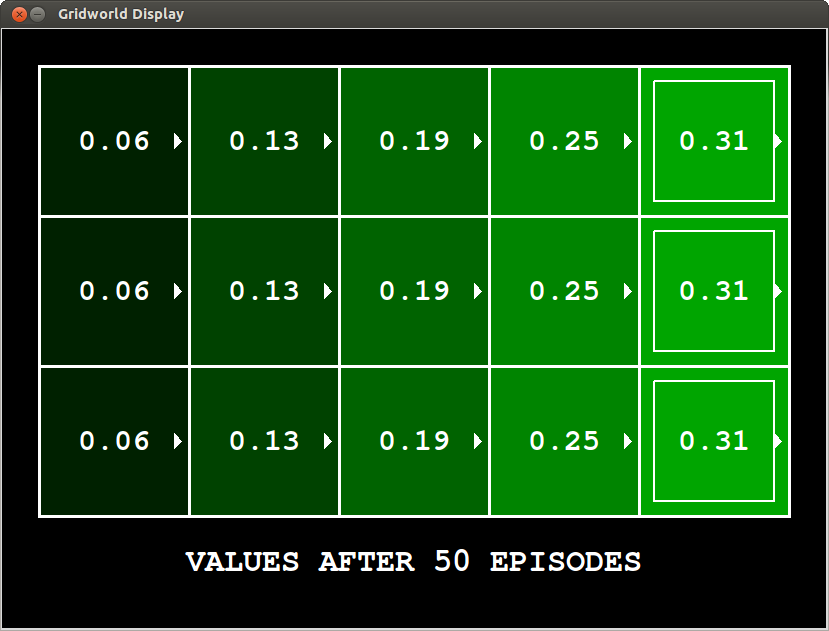
\includegraphics[width=\textwidth]{figure/sidewalk_v}
\end{subfigure}
\label{fig:rep}
\end{figure}

$\epsilon = 0.3, \gamma = 0.5$.
\texttt{{'bias': -0.20931133310480204, 'dis': 0.06742681562641269}}

\begin{figure}[h!]
\centering
\begin{subfigure}{0.49\textwidth}
	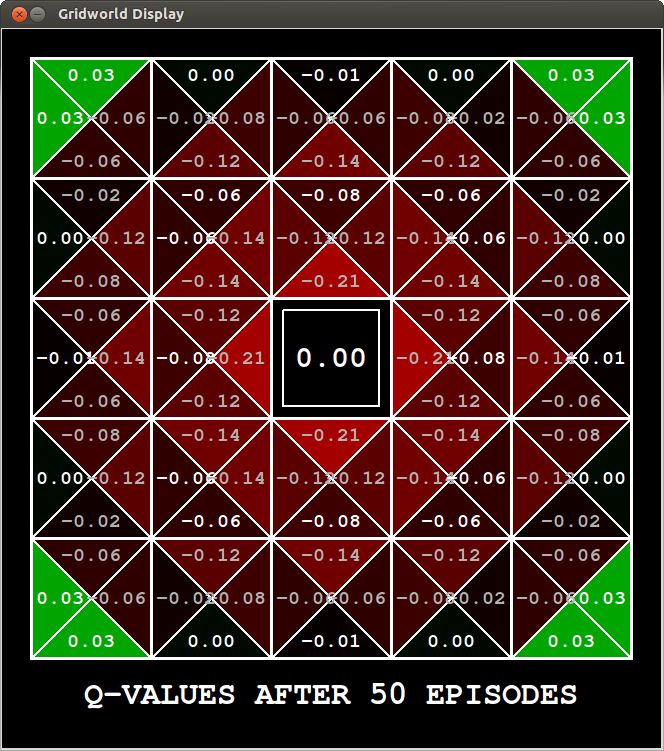
\includegraphics[width=\textwidth]{figure/obstacle}
\end{subfigure}
\begin{subfigure}{0.49\textwidth}
	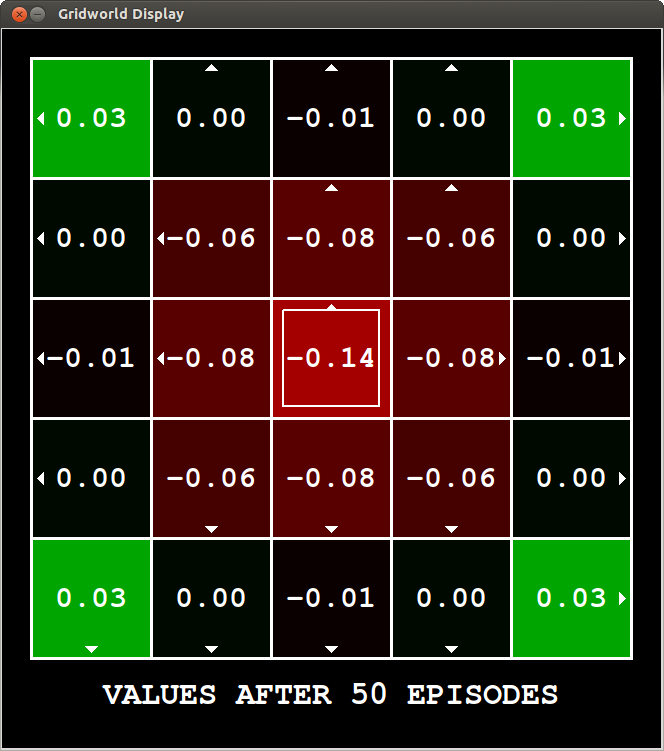
\includegraphics[width=\textwidth]{figure/obstacle_policy}
\end{subfigure}
\label{fig:rep}
\end{figure}

$\epsilon = 0.3, \gamma = 0.9$.
\texttt{{'x': 0.06250000371801567}}

\begin{figure}[h!]
\centering
\begin{subfigure}{0.9\textwidth}
	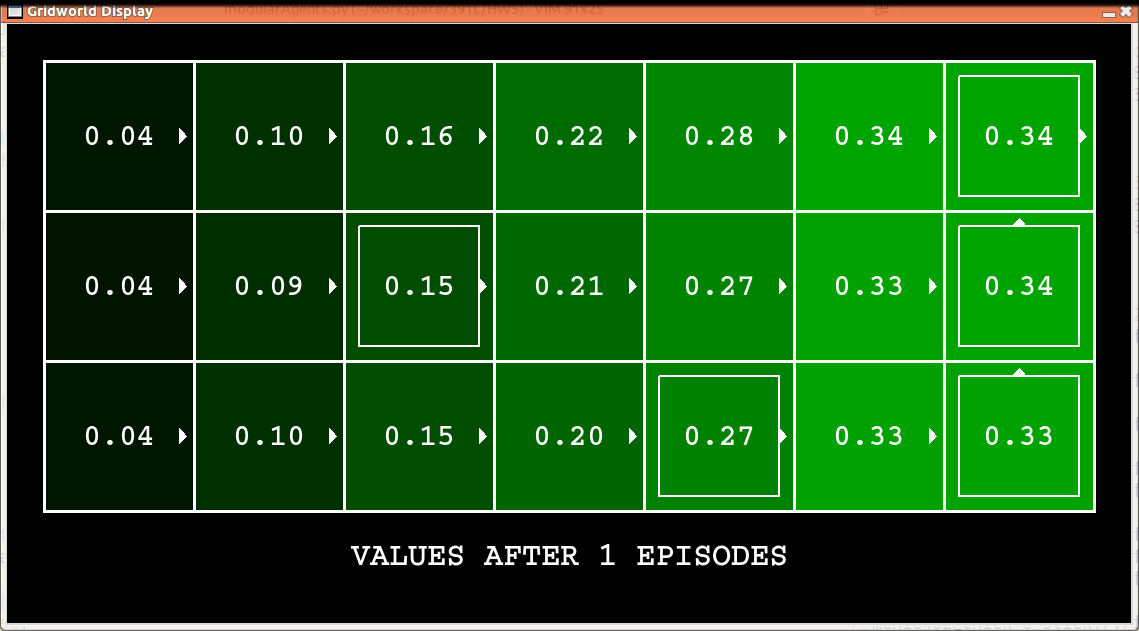
\includegraphics[width=\textwidth]{figure/hybird_walk}
\end{subfigure}
\begin{subfigure}{0.9\textwidth}
	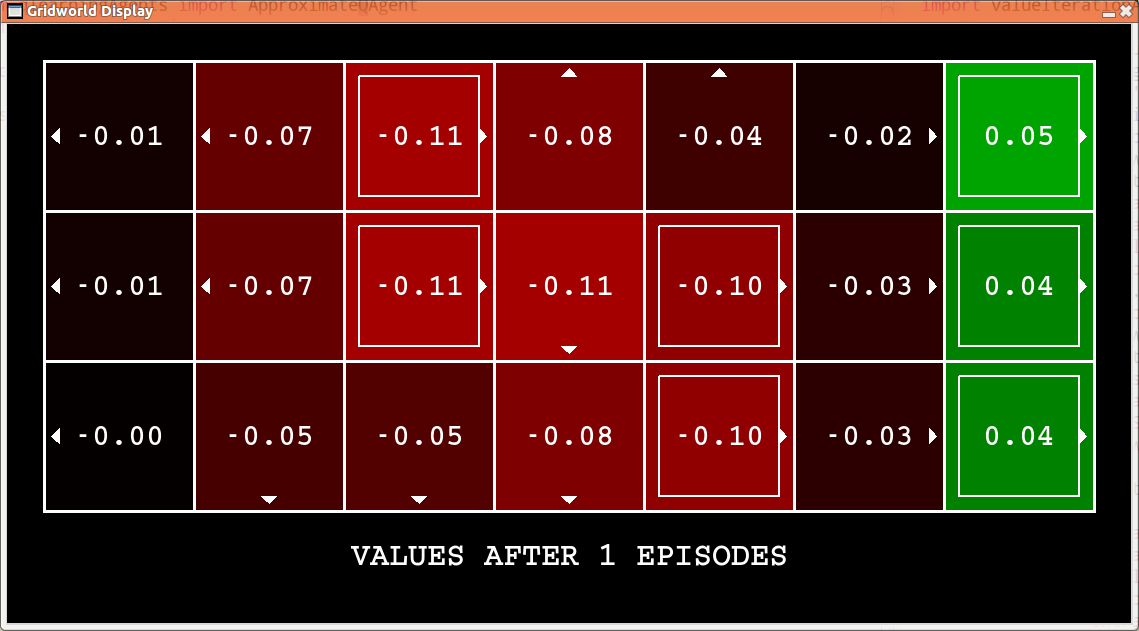
\includegraphics[width=\textwidth]{figure/hybird_obstacle}
\end{subfigure}
\label{fig:rep}
\end{figure}

\subsection{Hybird MDP: Linear Combination}

\begin{figure}[h!]
\centering
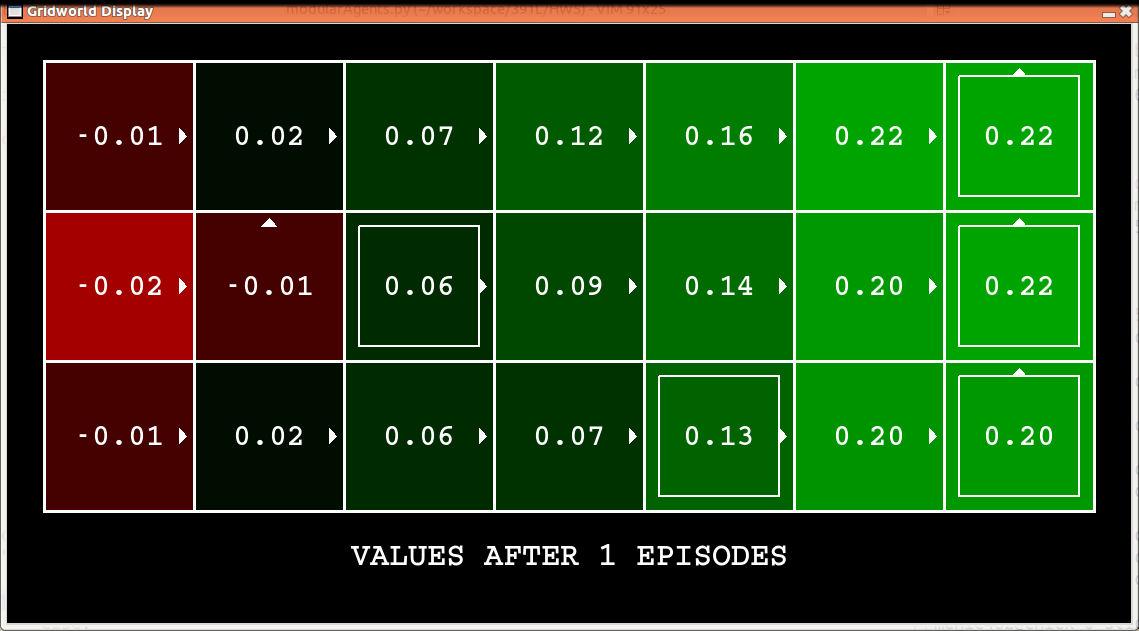
\includegraphics[width=\textwidth]{figure/hybird_6_4}
\end{figure}

\subsection{Hybird MDP: Gibbs Softmax}

\subsection{On Larger Grid}

\section{Discussion}

\end{document}
